% =============================================================================
%  FIVUCSAS — Poster variant: INFOGRAPHIC / DATA-VIZ
%  A0 portrait. Chart-heavy, big numbers, isotype icon grids, minimal prose.
%  Compile:  pdflatex poster.tex && pdflatex poster.tex
% =============================================================================
\documentclass[a0paper,portrait]{tikzposter}
\tikzposterlatexaffectionproofoff
\geometry{paperwidth=841mm,paperheight=1189mm}

\usepackage[utf8]{inputenc}
\usepackage[T1]{fontenc}
\usepackage{lmodern}
\renewcommand{\familydefault}{\sfdefault}
\usepackage{microtype}
\usepackage{xcolor}
\usepackage{graphicx}
\graphicspath{{../../assets/}{./assets/}{./poster/assets/}}
\usepackage{fontawesome5}
\usepackage{qrcode}
\usepackage{tikz}
\usepackage{enumitem}
\usepackage{array}
\usetikzlibrary{positioning,calc,arrows.meta,backgrounds,patterns,shapes.geometric}

% Official institutional crests (assets/)
\newcommand{\unicrest}[1][2.6cm]{
\includegraphics[height=#1,keepaspectratio]{marmara-university.png}}
\newcommand{\faccrest}[1][2.6cm]{
\includegraphics[height=#1,keepaspectratio]{muhendislik-fakultesi.jpg}}

% ---------- Vibrant palette --------------------------------------------------
\definecolor{IBg}{HTML}{F6F8FB}
\definecolor{INavy}{HTML}{0B2545}
\definecolor{ITeal}{HTML}{1E96A8}
\definecolor{IGold}{HTML}{F4B400}
\definecolor{ICoral}{HTML}{E76F51}
\definecolor{IGreen}{HTML}{2A9D8F}
\definecolor{IRed}{HTML}{C0392B}
\definecolor{IInk}{HTML}{1B1F23}
\definecolor{IGray}{HTML}{8E959B}
\definecolor{IGrayLite}{HTML}{E9ECEF}

% ---------- Theme ------------------------------------------------------------
\definelayouttheme{Infogr}{
  \usecolorstyle[colorPalette=InfoPal]{Default}
  \usebackgroundstyle{Default}
  \usetitlestyle{Filled}
  \useblockstyle{Default}
  \useinnerblockstyle{Default}
  \usenotestyle{Default}
}
\definecolorpalette{InfoPal}{
  \definecolor{colorOne}{named}{INavy}
  \definecolor{colorTwo}{named}{ITeal}
  \definecolor{colorThree}{named}{IGold}
}
\usetheme{Infogr}
\colorlet{backgroundcolor}{IBg}
\colorlet{framecolor}{INavy}
\colorlet{titlefgcolor}{white}
\colorlet{titlebgcolor}{INavy}
\colorlet{blocktitlebgcolor}{ITeal}
\colorlet{blocktitlefgcolor}{white}
\colorlet{blockbodybgcolor}{white}
\colorlet{blockbodyfgcolor}{IInk}
\colorlet{innerblocktitlebgcolor}{IGold}
\colorlet{innerblocktitlefgcolor}{INavy}

% ---------- Pictogram helper (icon repeated) --------------------------------
\newcommand{\picto}[3]{% color, icon, count
  \foreach \i in {1,...,#3}{\textcolor{#1}{#2}}}

% ---------- Title ------------------------------------------------------------
\title{\parbox{0.96\linewidth}{\centering
  \begin{minipage}[c]{0.11\linewidth}\centering\unicrest[2.6cm]\end{minipage}\hfill
  \begin{minipage}[c]{0.74\linewidth}\centering
  {\fontsize{96}{96}\selectfont\bfseries FIVUCSAS}\\[0.10em]
  \Large Face and Identity Verification Using Cloud-based SaaS\\[0.20em]
  \normalsize\textsl{The numbers behind a multi-tenant biometric auth platform}
  \end{minipage}\hfill
  \begin{minipage}[c]{0.11\linewidth}\centering\faccrest[2.8cm]\end{minipage}
}}
\author{\large
  \textbf{Ahmet Abdullah Gültekin} \quad
  \textbf{Ayşe Gülsüm Eren} \quad
  \textbf{Ayşenur Arıcı}\\[0.2em]
  \normalsize Advisor: Assoc.\ Prof.\ Dr.\ Mustafa Ağaoğlu \, · \, CSE4197 / CSE4198 \, · \, Spring 2025–2026}
\institute{Marmara University \, · \, Faculty of Engineering \, · \, Department of Computer Engineering}

\begin{document}
\maketitle[width=\paperwidth, titletotopverticalspace=6mm]

% =============================================================================
% GIANT KPI ROW
% =============================================================================
\block[bodyoffsety=-15mm, bodyinnersep=5mm]{}{%
\centering
\begin{tikzpicture}[every node/.style={align=center}]
  % KPI 1: 0% with thumbs up
  \node[font=\fontsize{120}{120}\selectfont\bfseries, text=IGreen] at (-22,0.5) {0\%};
  \node[font=\Large, text=IInk] at (-22,-3.5) {\bfseries Replay-attack false-accept};
  \node[font=\small, text=IGray] at (-22,-4.5) {n = 120 recorded-video attempts};

  % KPI 2: <1s
  \node[font=\fontsize{120}{120}\selectfont\bfseries, text=ITeal] at (0,0.5) {<\!1s};
  \node[font=\Large, text=IInk] at (0,-3.5) {\bfseries End-to-end verification};
  \node[font=\small, text=IGray] at (0,-4.5) {P95 = 950 ms, CPU only};

  % KPI 3: 10 with pictograms
  \node[font=\fontsize{120}{120}\selectfont\bfseries, text=IGold] at (22,0.5) {10};
  \node[font=\Large, text=IInk] at (22,-3.5) {\bfseries Composable auth factors};
  \node[font=\small, text=IGray] at (22,-4.5) {any subset → MFA flow per tenant};

  \draw[draw=IGray, line width=0.6pt] (-11,-5.0) -- (-11,3.0);
  \draw[draw=IGray, line width=0.6pt] ( 11,-5.0) -- ( 11,3.0);
\end{tikzpicture}}

% =============================================================================
% HERO PANEL: 3 visual takeaways stacked
% =============================================================================
\block[titleoffsety=-10mm, bodyinnersep=6mm]{At a glance}{%
\centering
\begin{tikzpicture}[every node/.style={font=\normalsize}]

% ---------- LEFT: stacked attack-defeat pictograms -------------------------
\begin{scope}[shift={(-22,0)}]
  \node[font=\Large\bfseries, text=INavy] at (0,5.2) {Attacks defeated};
  \node[font=\small, text=IGray, align=center, text width=14cm] at (0,4.4)
       {each icon = a confirmed defeat in our test bench};

  % photo replay - bank of 12 phones, all green (defeated)
  \node[anchor=west, font=\large, text=IInk] at (-7.5,3.2) {\bfseries Photo on screen};
  \node[anchor=east, font=\Large\bfseries, text=IGreen] at (7.5,3.2) {30\,/\,30};
  \node[anchor=west, text=IGreen] at (-7.5,2.4) {\large\picto{IGreen}{\faMobile}{30}};

  % video replay
  \node[anchor=west, font=\large, text=IInk] at (-7.5,1.4) {\bfseries Recorded video};
  \node[anchor=east, font=\Large\bfseries, text=IGreen] at (7.5,1.4) {60\,/\,60};
  \node[anchor=west, text=IGreen] at (-7.5,0.6) {\large\picto{IGreen}{\faVideo}{60}};

  % printed photo
  \node[anchor=west, font=\large, text=IInk] at (-7.5,-0.4) {\bfseries Printed photo};
  \node[anchor=east, font=\Large\bfseries, text=IGreen] at (7.5,-0.4) {15\,/\,15};
  \node[anchor=west, text=IGreen] at (-7.5,-1.2) {\large\picto{IGreen}{\faImage}{15}};

  % 3d mask (still attempted, harder)
  \node[anchor=west, font=\large, text=IInk] at (-7.5,-2.2) {\bfseries Static 3D mask};
  \node[anchor=east, font=\Large\bfseries, text=IGold] at (7.5,-2.2) {13\,/\,15};
  \node[anchor=west] at (-7.5,-3.0)
     {{\color{IGold}\large\picto{IGold}{\faTheaterMasks}{13}}{\color{IGray}\large\picto{IGray}{\faTheaterMasks}{2}}};

  % deepfake stream
  \node[anchor=west, font=\large, text=IInk] at (-7.5,-4.0) {\bfseries Deepfake stream};
  \node[anchor=east, font=\Large\bfseries, text=ICoral] at (7.5,-4.0) {ongoing};
  \node[anchor=west, text=ICoral] at (-7.5,-4.8) {\large\faExclamationTriangle\ \small\textit{Defended by sequence-mismatch heuristic; under continued red-team}};
\end{scope}

% ---------- MIDDLE: latency donut -----------------------------------------
\begin{scope}[shift={(0,0)}]
  \node[font=\Large\bfseries, text=INavy] at (0,5.2) {Latency budget};
  \node[font=\small, text=IGray] at (0,4.4) {P95 end-to-end face verification = 950 ms};

  % donut: arcs proportional to ms; total=950
  % shares (deg out of 360): emb 240/950=90.9, anti 210=79.6, db 200=75.8, mesh 180=68.2, det 120=45.5
  \def\R{4.0}\def\r{2.2}
  \def\sA{0}    \def\eA{90.9}
  \def\sB{90.9} \def\eB{170.5}
  \def\sC{170.5}\def\eC{246.3}
  \def\sD{246.3}\def\eD{314.5}
  \def\sE{314.5}\def\eE{360}
  \fill[ITeal]  (0,0) -- ({\R*cos(\sA)},{\R*sin(\sA)}) arc (\sA:\eA:\R) -- cycle;
  \fill[IGold]  (0,0) -- ({\R*cos(\sB)},{\R*sin(\sB)}) arc (\sB:\eB:\R) -- cycle;
  \fill[ICoral] (0,0) -- ({\R*cos(\sC)},{\R*sin(\sC)}) arc (\sC:\eC:\R) -- cycle;
  \fill[INavy]  (0,0) -- ({\R*cos(\sD)},{\R*sin(\sD)}) arc (\sD:\eD:\R) -- cycle;
  \fill[IGreen] (0,0) -- ({\R*cos(\sE)},{\R*sin(\sE)}) arc (\sE:\eE:\R) -- cycle;
  \fill[white]  (0,0) circle (\r);
  \node[font=\fontsize{32}{32}\selectfont\bfseries, text=INavy] at (0,0.3) {950};
  \node[font=\small, text=IGray] at (0,-0.7) {ms total};

  % legend
  \def\lyo{-5.0}
  \node[fill=ITeal,  minimum width=0.6cm, minimum height=0.6cm] (lt1) at (-6, \lyo+1.0)  {};
  \node[anchor=west, font=\small, text=IInk] at (-5.5, \lyo+1.0) {Embedding (Facenet512)  240 ms};
  \node[fill=IGold,  minimum width=0.6cm, minimum height=0.6cm] (lt2) at (-6, \lyo+0.2)  {};
  \node[anchor=west, font=\small, text=IInk] at (-5.5, \lyo+0.2) {Anti-spoof (UniFace)    210 ms};
  \node[fill=ICoral, minimum width=0.6cm, minimum height=0.6cm] (lt3) at (-6, \lyo-0.6)  {};
  \node[anchor=west, font=\small, text=IInk] at (-5.5, \lyo-0.6) {DB search (HNSW)        200 ms};
  \node[fill=INavy,  minimum width=0.6cm, minimum height=0.6cm] (lt4) at (-6, \lyo-1.4)  {};
  \node[anchor=west, font=\small, text=IInk] at (-5.5, \lyo-1.4) {Face mesh (468 pt)      180 ms};
  \node[fill=IGreen, minimum width=0.6cm, minimum height=0.6cm] (lt5) at (-6, \lyo-2.2)  {};
  \node[anchor=west, font=\small, text=IInk] at (-5.5, \lyo-2.2) {Face detection (MTCNN)  120 ms};
\end{scope}

% ---------- RIGHT: codebase by-the-numbers --------------------------------
\begin{scope}[shift={(22,0)}]
  \node[font=\Large\bfseries, text=INavy] at (0,5.2) {The codebase};
  \node[font=\small, text=IGray] at (0,4.4) {by the numbers, 2026-05};

  % big tile rows
  \node[fill=INavy, text=IGold, minimum width=14cm, minimum height=1.8cm,
        rounded corners=4pt, font=\Large\bfseries] at (0,3.0) {1\,820+ tests};
  \node[font=\small, text=IGray] at (0,1.9) {633 Java + 619 web + 425 mobile + 114 spoof-detector + 27 Playwright};

  \node[fill=ITeal, text=white, minimum width=6.8cm, minimum height=1.6cm,
        rounded corners=4pt, font=\Large\bfseries] at (-3.6, 0.4) {5 services};
  \node[fill=IGold, text=INavy, minimum width=6.8cm, minimum height=1.6cm,
        rounded corners=4pt, font=\Large\bfseries] at ( 3.6, 0.4) {60 migrations};

  \node[fill=ICoral, text=white, minimum width=6.8cm, minimum height=1.6cm,
        rounded corners=4pt, font=\Large\bfseries] at (-3.6,-1.5) {8 ADRs};
  \node[fill=IGreen, text=white, minimum width=6.8cm, minimum height=1.6cm,
        rounded corners=4pt, font=\Large\bfseries] at ( 3.6,-1.5) {1 CX43 VPS};

  \node[font=\small, text=IGray, align=center, text width=14cm] at (0,-2.8)
       {Hetzner Cloud · 8 CPU · 16 GB RAM · 150 GB · Ubuntu 24.04};
  \node[font=\small, text=IGray, align=center, text width=14cm] at (0,-3.5)
       {Docker 29.3.0 · Traefik 3.6 · Postgres 17 + pgvector · Redis 7.4};
\end{scope}

\end{tikzpicture}}

% =============================================================================
% CONTRIBUTIONS BAR
% =============================================================================
\block{Contributions}{%
\centering\small
\begin{tikzpicture}[every node/.style={align=center, font=\small},
  cbox/.style={draw=INavy, line width=0.5pt, fill=white, rounded corners=4pt,
               minimum width=7.0cm, minimum height=3.6cm, text width=6.4cm}]
\node[cbox] at (-19.5,0) {\textbf{\color{INavy}C1.}\\ Tenant-configurable composition of \textbf{10 auth factors} into MFA flows declared at admin layer.};
\node[cbox] at (-12.5,0) {\textbf{\color{INavy}C2.}\\ Active randomised \textbf{liveness} — n-step facial-action sequence bound to a per-attempt nonce.};
\node[cbox] at ( -5.5,0) {\textbf{\color{INavy}C3.}\\ Pipeline decomposition along the \textbf{OIDC / ML iteration} boundary, two services on private network.};
\node[cbox] at (  5.5,0) {\textbf{\color{INavy}C4.}\\ Embedding-at-rest \textbf{Fernet encryption} (AES-128-CBC + HMAC-SHA-256) prior to pgvector write.};
\node[cbox] at ( 12.5,0) {\textbf{\color{INavy}C5.}\\ Regulator-aware data lifecycle — \textbf{GDPR Art.\ 15 / 17} and KVKK soft-delete + purge + audit.};
\node[cbox] at ( 19.5,0) {\textbf{\color{INavy}M.}\\ Per-attempt method — server issues nonce, client streams 60 frames, server checks EAR/MAR/yaw + spoof.};
\end{tikzpicture}}

% =============================================================================
% AUTH FACTORS — isotype grid full width
% =============================================================================
\block{10 composable factors}{%
\centering
\begin{tikzpicture}[every node/.style={font=\small, text=IInk, align=center},
  tile/.style={draw=INavy, line width=0.5pt, fill=white, rounded corners=3pt,
               minimum width=6.5cm, minimum height=2.5cm, align=center},
  gtile/.style={draw=IGold, fill=IGold!20, line width=0.8pt, rounded corners=3pt,
               minimum width=6.5cm, minimum height=2.5cm, align=center}]
\node[tile]  at (-21, 1.5) {\fontsize{26}{26}\selectfont\faKey\\[1mm]\bfseries Password};
\node[tile]  at (-14, 1.5) {\fontsize{26}{26}\selectfont\faEnvelope\\[1mm]\bfseries Email OTP};
\node[tile]  at ( -7, 1.5) {\fontsize{26}{26}\selectfont\faSms\\[1mm]\bfseries SMS OTP};
\node[tile]  at (  0, 1.5) {\fontsize{26}{26}\selectfont\faClock\\[1mm]\bfseries TOTP};
\node[tile]  at (  7, 1.5) {\fontsize{26}{26}\selectfont\faQrcode\\[1mm]\bfseries QR code};
\node[gtile] at ( 14, 1.5) {\fontsize{26}{26}\selectfont\faSmile\\[1mm]\bfseries Face};
\node[gtile] at ( 21, 1.5) {\fontsize{26}{26}\selectfont\faMicrophone\\[1mm]\bfseries Voice};
\node[gtile] at (-14,-1.7) {\fontsize{26}{26}\selectfont\faFingerprint\\[1mm]\bfseries Fingerprint};
\node[tile]  at ( -7,-1.7) {\fontsize{26}{26}\selectfont\faUsb\\[1mm]\bfseries WebAuthn};
\node[tile]  at (  0,-1.7) {\fontsize{26}{26}\selectfont\faIdCard\\[1mm]\bfseries NFC document};
\node[anchor=west, font=\large, text=IInk] at (4,-1.7)
     {\textcolor{IGold}{\rule{0.5cm}{0.5cm}}\ \textbf{gold} = active-liveness wrapped};
\end{tikzpicture}}

% =============================================================================
% ARCHITECTURE & PROBLEM/SOLUTION COLUMNS
% =============================================================================
\begin{columns}

\column{0.5}
\block{Why active liveness}{%
\centering\small
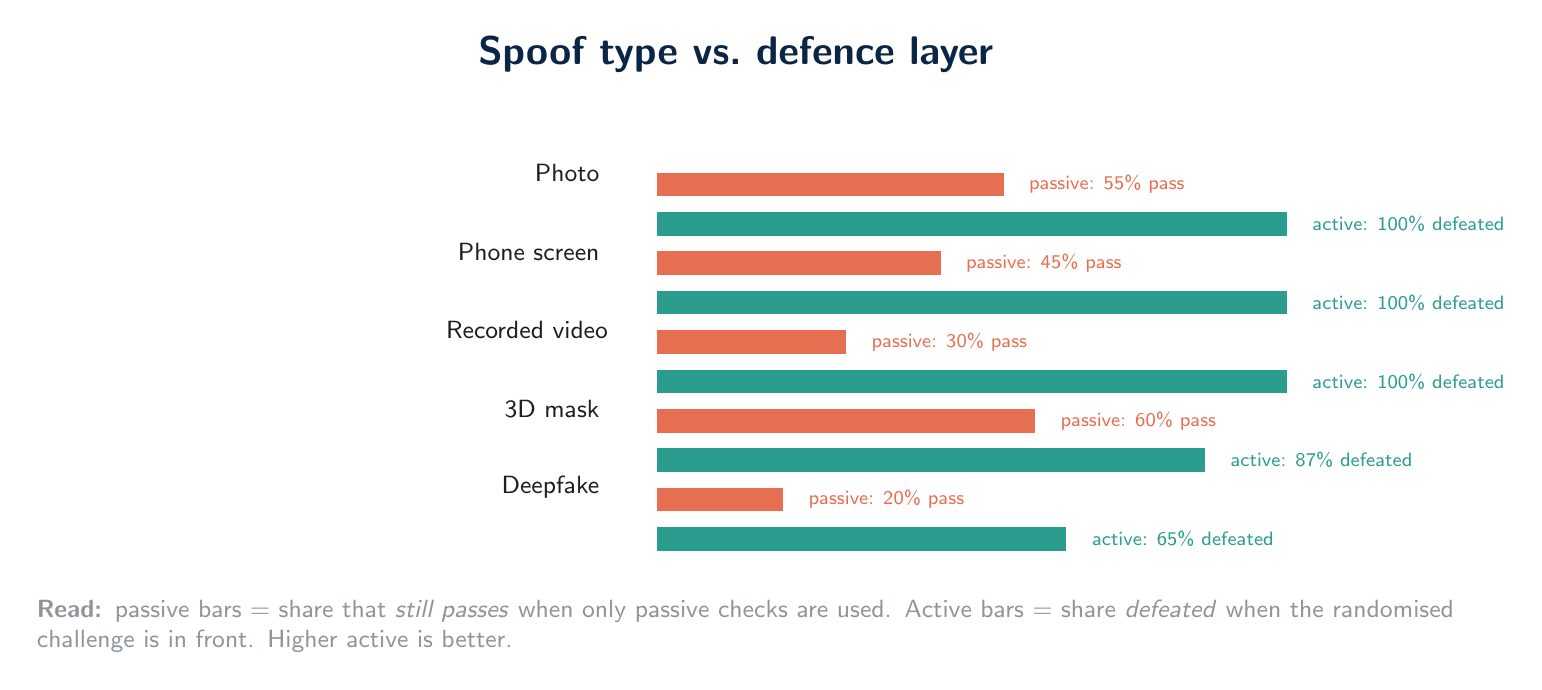
\begin{tikzpicture}[every node/.style={align=center}]
% bar comparison
\def\W{16}
\node[font=\Large\bfseries, text=INavy] at (0,5.5) {Spoof type vs.\ defence layer};
% rows
\foreach \i/\name/\pf/\pct/\af/\afct in {%
  0/{Photo}        /0.55/55/1.00/100,
  1/{Phone screen} /0.45/45/1.00/100,
  2/{Recorded video}/0.30/30/1.00/100,
  3/{3D mask}      /0.60/60/0.87/87,
  4/{Deepfake}     /0.20/20/0.65/65}{
  \pgfmathsetmacro{\y}{4 - \i*1.0}
  \node[anchor=east, font=\small, text=IInk] at (-1.5,\y) {\name};
  \filldraw[fill=ICoral, draw=none] (-1,\y-0.3) rectangle ({-1+8*\pf},\y+0.0);
  \node[anchor=west, font=\scriptsize, text=ICoral] at ({-1+8*\pf+0.2},\y-0.15)
       {passive: \pct\% pass};
  \filldraw[fill=IGreen, draw=none] (-1,\y-0.8) rectangle ({-1+8*\af},\y-0.5);
  \node[anchor=west, font=\scriptsize, text=IGreen] at ({-1+8*\af+0.2},\y-0.65)
       {active: \afct\% defeated};
}
\node[font=\small, text=IGray, align=left, text width=18cm, anchor=north west]
     at (-9,-1.3)
     {\textbf{Read:} passive bars = share that \emph{still passes} when only
      passive checks are used. Active bars = share \emph{defeated} when the
      randomised challenge is in front. Higher active is better.};
\end{tikzpicture}}

\column{0.5}
\block{System map}{%
\centering
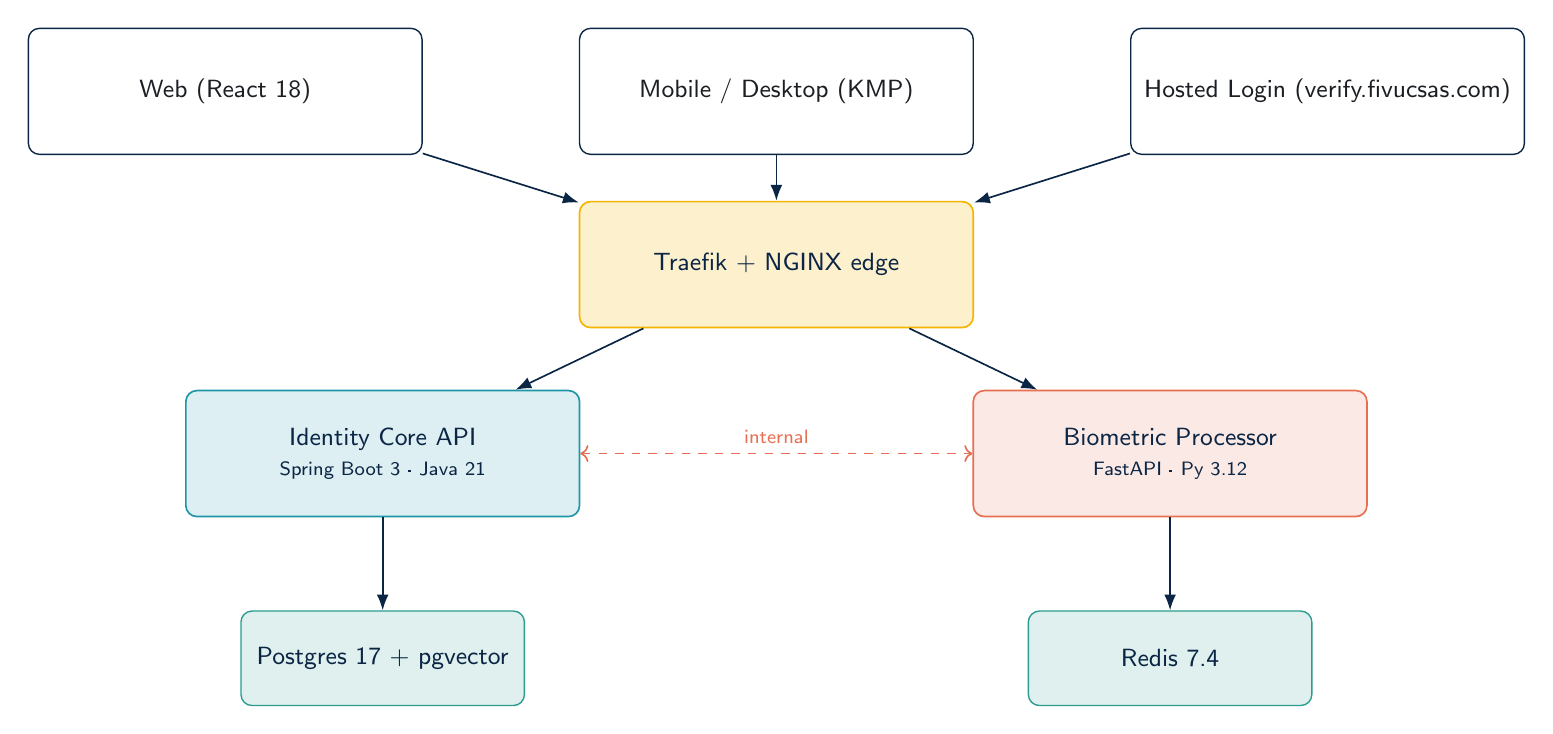
\begin{tikzpicture}[every node/.style={font=\small, text=IInk},
  client/.style={draw=INavy, fill=white, rounded corners=4pt, line width=0.5pt,
                 minimum width=5cm, minimum height=1.6cm, align=center},
  edge/.style={draw=IGold, fill=IGold!20, rounded corners=4pt, line width=0.6pt,
               minimum width=5cm, minimum height=1.6cm, align=center, text=INavy},
  svc/.style={draw=ITeal, fill=ITeal!15, rounded corners=4pt, line width=0.6pt,
              minimum width=5cm, minimum height=1.6cm, align=center, text=INavy},
  ml/.style ={draw=ICoral, fill=ICoral!15, rounded corners=4pt, line width=0.6pt,
              minimum width=5cm, minimum height=1.6cm, align=center, text=INavy},
  data/.style={draw=IGreen, fill=IGreen!15, rounded corners=4pt, line width=0.5pt,
              minimum width=3.6cm, minimum height=1.2cm, align=center, text=INavy},
  arrow/.style={-Latex, draw=INavy, line width=0.6pt}]
\node[client] (web)  at (-7,3.2) {Web (React 18)};
\node[client] (mob)  at ( 0,3.2) {Mobile / Desktop (KMP)};
\node[client] (hl)   at ( 7,3.2) {Hosted Login (verify.fivucsas.com)};
\node[edge]   (gw)   at (0,1.0)  {Traefik + NGINX edge};
\node[svc]    (api)  at (-5,-1.4){Identity Core API\\\scriptsize Spring Boot 3 · Java 21};
\node[ml]     (bio)  at ( 5,-1.4){Biometric Processor\\\scriptsize FastAPI · Py 3.12};
\node[data]   (db)   at (-5,-4.0){Postgres 17 + pgvector};
\node[data]   (rd)   at ( 5,-4.0){Redis 7.4};
\foreach \c in {web,mob,hl} {\draw[arrow] (\c) -- (gw);}
\draw[arrow] (gw) -- (api); \draw[arrow] (gw) -- (bio);
\draw[arrow] (api) -- (db); \draw[arrow] (bio) -- (rd);
\draw[arrow, <->, dashed, draw=ICoral] (api) -- node[above,sloped,font=\scriptsize,text=ICoral]{internal} (bio);
\end{tikzpicture}\par\vspace{2mm}
\small\textit{Biometric service has no public route — Docker network only, API-key gated.}}

\end{columns}

% =============================================================================
% CONCLUSION BAR
% =============================================================================
\block{Conclusion}{\centering\normalsize
\parbox{0.95\linewidth}{\centering\itshape
Production-grade, GDPR-compliant biometric authentication \emph{is} achievable on commodity
hardware when the system is decomposed along its right axis — a frozen OIDC contract on one
side, an iterating ML pipeline on the other — and when liveness is treated as an active,
challenge-driven property rather than a passive signal alone. Measured \textbf{0 / 120
replay-attack false-accepts} and \textbf{0.97 passive-spoof AUC} are both within practical
deployment limits on a single CPU server.}}

% =============================================================================
% FOOTER ROW — qr + future work + footer
% =============================================================================
\block{Live demo \& what's next}{%
\begin{minipage}[t]{0.22\linewidth}\centering
\qrcode[height=4.6cm,version=4,level=H]{https://verify.fivucsas.com}\\[2mm]
\small\faCamera\ \textbf{Scan to test it}\\
\small\texttt{verify.fivucsas.com}
\end{minipage}\hfill
\begin{minipage}[t]{0.36\linewidth}\small\color{IInk}
\textbf{\color{INavy}Future work}
\begin{itemize}[leftmargin=*, label=\textcolor{IGold}{\textbf{→}}, nosep]
\item BYOD tenant DB — tenants host biometric data themselves
\item On-device pre-filter — bandwidth + privacy win
\item Cross-modal challenge — voice nonce + facial action
\item W3C verifiable credentials post-KYC
\end{itemize}
\end{minipage}\hfill
\begin{minipage}[t]{0.36\linewidth}\footnotesize\color{IInk}
\textbf{\color{INavy}References}
\begin{enumerate}[leftmargin=*, label={[\arabic*]}, nosep]
\item Serengil, S., Özpınar, A. \textit{LightFace / DeepFace}. IEEE ASYU, 2020.
\item Lugaresi, C.\ et al. \textit{MediaPipe.} arXiv:1906.08172.
\item Soukupová, T., Čech, J. \textit{Real-Time Eye Blink Detection.} CVWW, 2016.
\item Wan, L.\ et al. \textit{Generalized End-to-End Loss for Speaker Verification.} ICASSP, 2018.
\item Yadav, S.\ et al. \textit{UniFace.} CVPR-W, 2023.
\end{enumerate}
\end{minipage}}

% Footer ---------------------------------------------------------------------
\block[bodyinnersep=2mm, bodyverticalshift=0mm]{}{%
\colorbox{INavy}{\parbox{0.985\linewidth}{\centering\color{IGold}%
\vspace{2mm}\bfseries\small
\faGithub\ \texttt{github.com/Rollingcat-Software/FIVUCSAS}
\quad·\quad
\faGlobe\ \texttt{fivucsas.com}
\quad·\quad
\faEnvelope\ \texttt{ahmetabdullahgultekin@gmail.com}
\quad·\quad
Marmara University \textbf{2026}\vspace{2mm}}}}

\end{document}
